\section{Experimental Results}
\frame
{
\frametitle{Experimental Results}
\framesubtitle{}
\begin{itemize}
	\item AMD Athlon 2500+ CPU
	\item 512M RAM
	\item NVidia GeForce 6800GT GPU
	\item Colville minimization problem as benchmark.
	$$f(\bar{x}) = 100\cdot(x_{1}^{2} - x_{2})^{2} + (1-x_{1})^{2} + 90\cdot (x_{3}^{2} - x_{4})^{2} + (1 -x_{3})^{2}$$ 
	$$+ 10.1\cdot((1-x_{2})^{2} + (1-x_{4})^{2}) + 19.8\cdot (x_{2} -1)(x_{4} - 1)$$
	\item where $-18 \leq x_{i} \leq 10,\ i = 1,2,3,4$ with the global solution $(1,1,1,1)$ and $f(1,1,1,1)=0$.
\end{itemize}
}

\frame
{
\frametitle{Experimental Results}
\framesubtitle{}
\begin{center}
	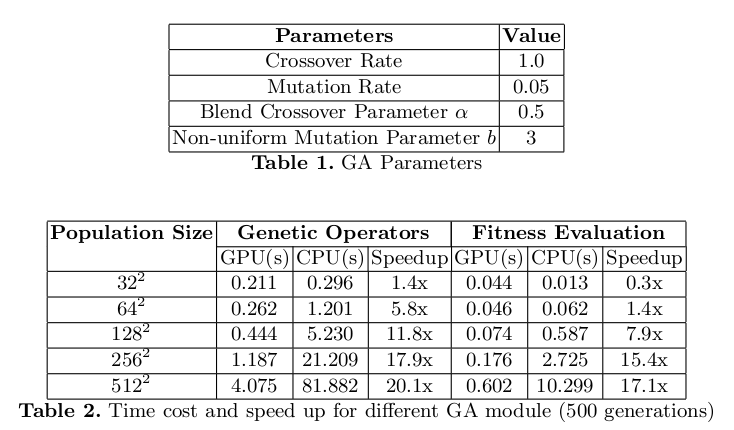
\includegraphics[width=0.8\textwidth]{img/tables}
\end{center}
}

\frame
{
\frametitle{Experimental Results}
\framesubtitle{}
\begin{center}
	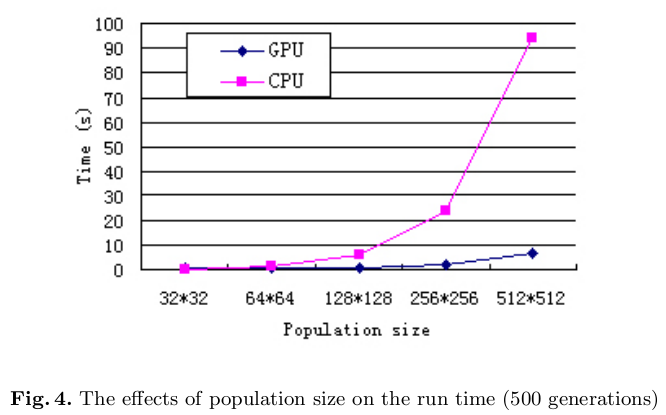
\includegraphics[width=0.8\textwidth]{img/grafico}
\end{center}
}
